\subsection{Research Object-Enabled myExperiment}
\label{sec:myexperiment}

%This section describes the efforts that went into incorporating research objects within myExperiment. In particular, how the notion of myExperiment pack was used as a starting point to incorporate new features/functionalaities. We will also discuss the diferent iterations that involved Wf4ever and Biovel users in those developments.

In this section, we describe how myExperiment \cite{DBLP:journals/fgcs/RoureGS09} was extended in order to cater for the sharing, publication and curation of Research Objects. myExperiment is a virtual research environment targeted towards collaborations for sharing and publishing workflows (and experiments). It provides the functionalities necessary for sharing workflows within and across multiple communities. In doing so, myExperiment adopts a social web approach, which is adapted to the need of scientists. The workflows that are shared using myExperiment do not need to be specified in a particular workflow management system. For example, we find on myExpeirment workflows that have been specified using Galaxy \cite{galaxy}, Taverna \cite{taverna}, Kepler \cite{kepler} and Vistrails \cite{vistrails}.

\begin{figure}
\begin{center}
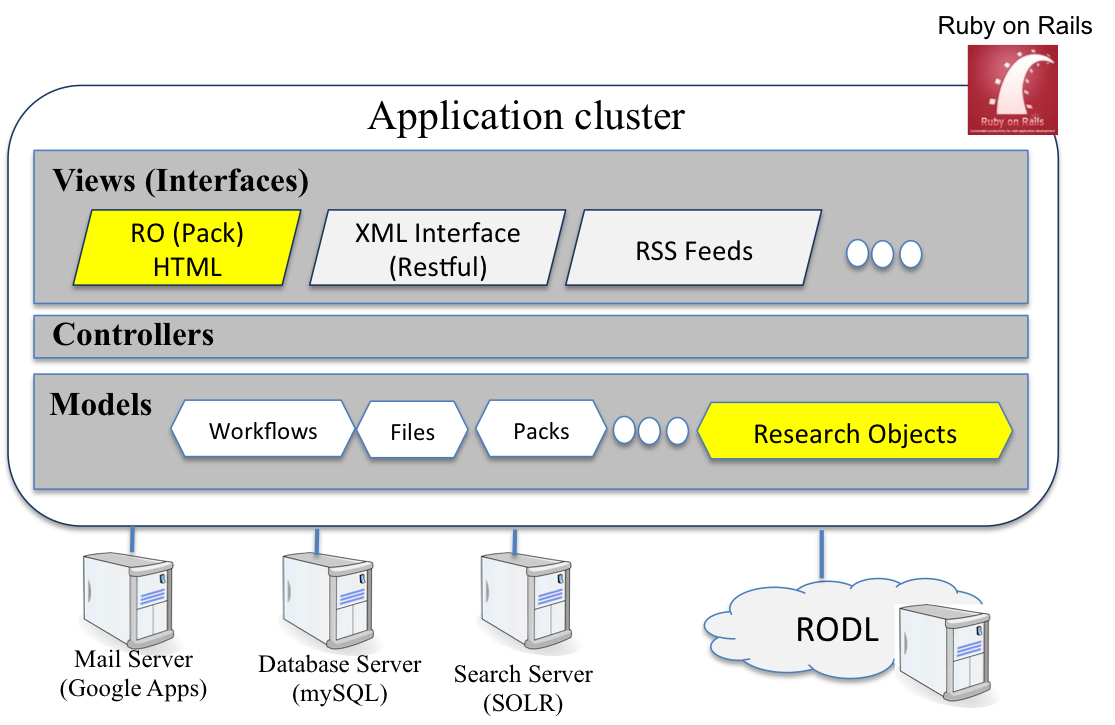
\includegraphics[width=0.7\textwidth]{Figures/myexperimentArchitecture.png}
\end{center}
\caption{RO-enabled myExperiment (except RODL, the modules in the above figure belong to the myExperiment infrastructure).}
\label{fig:myexperimentarchitecture}
\end{figure}


While initially targeted towards workflows, the creators of myExperiment were aware that scientists wants to share more than just workflows and experiments. Because of this, myExperiemnt was extended to support the sharing of artifacts known as Packs. A pack can be seen as a basic aggregation of resources, which can be workflows, but also files, presentations, papers, or links to external resources. 
The notion of packs have been widely adopted by scientists. At the time of writing, myExperiment had $337$ packs. Just like a workflow, using myExperiment a pack can be annotated and shared. 
 
\begin{figure}
\begin{center}
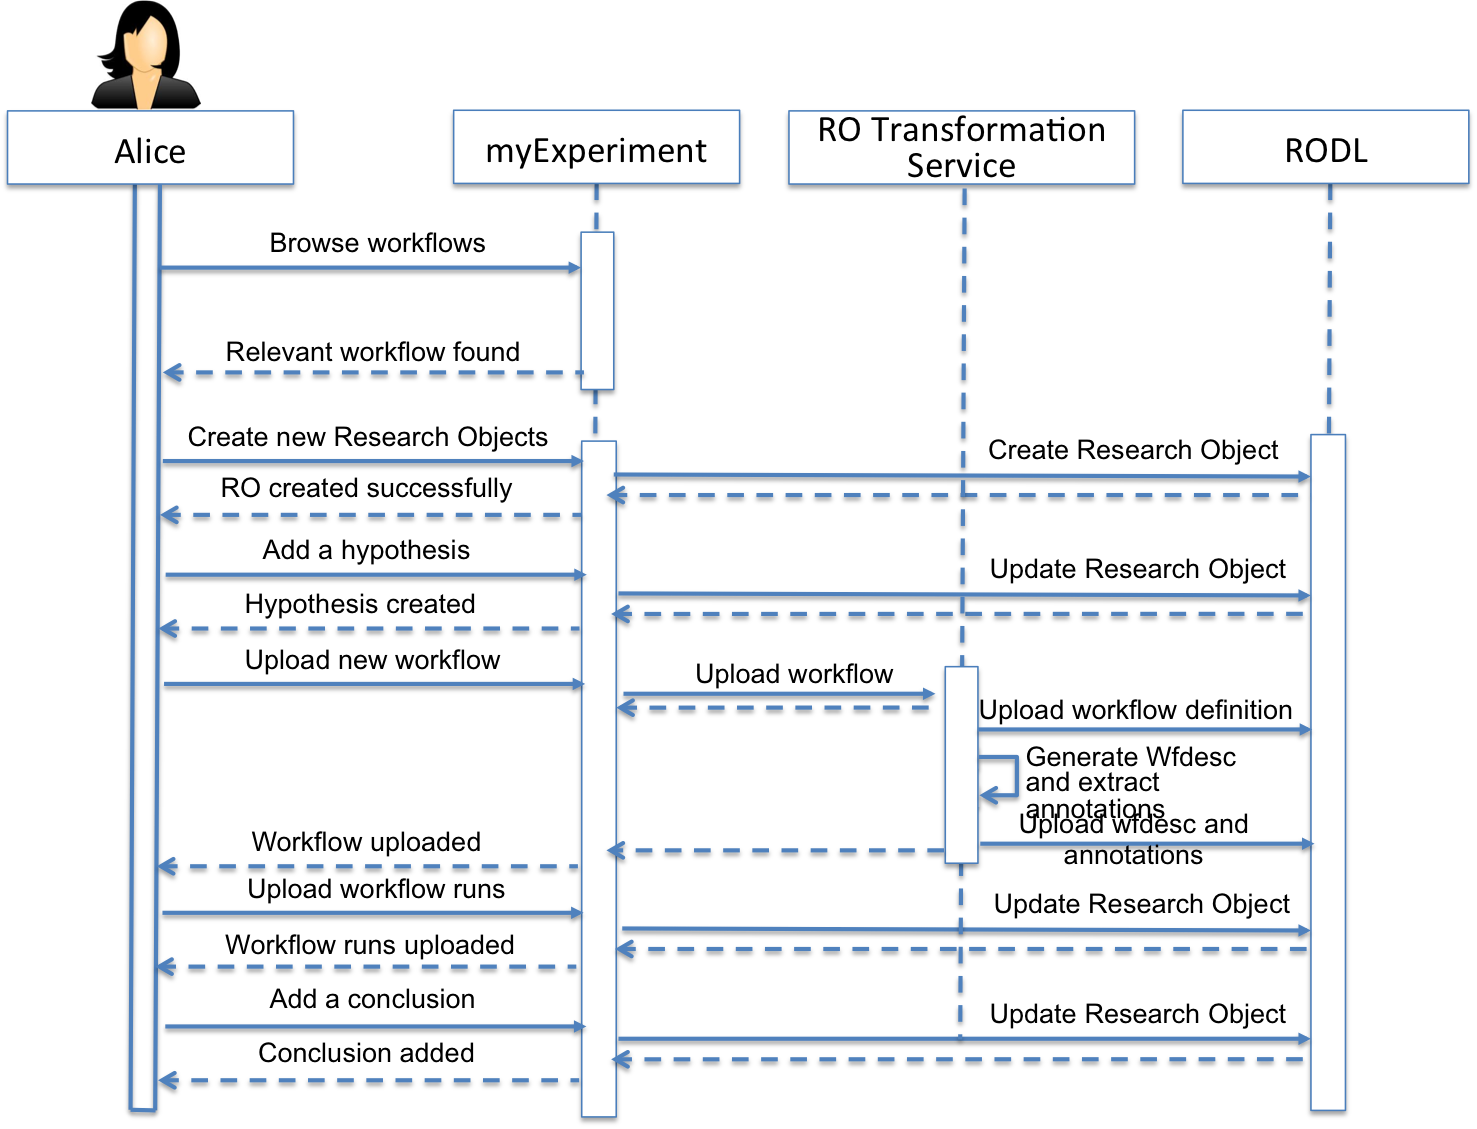
\includegraphics[width=0.7\textwidth]{Figures/myexperimentInteractions.png}
\end{center}
\caption{A Sequence diagram illustrating how myExperiment can be used to create Research Objects.}
\label{fig:myexperimentinteractions}
\end{figure} 
 
In order to support complex forms of sharing, reuse and preservation, we have worked during the last year on incorporating the notion of Research Objects (which can be seen as advanced packs) into the development version of myExperiment \footnote{http://alpha.myexperiment.org/packs/}. In addition to the basic aggregation supported by packs, alpha myExperiment\footnote{It is worth noting that once the development in the myExperiment alpha is judged mature, the new functionalities will be staged to the production version of myExperiment.} provides the mechanisms for specifying metadata that describes the relationships between the resources within the aggregation. Moreover, the structure and the types of the resources that compose a pack are now inline with those that have been identifying thanks to the Research Object model. For example, a user is able to specify that a given file within a pack specifies the hypothesis, that another file specifies the workflow run obtained by enacting a given workflow, or that a given file states the conclusions drew by the scientists after analyzing the workflow run.


Figure \ref{fig:myexperimentarchitecture} illustrates a high-level architecture of Alpha myExpeirment, the development version of myExperiment into which the Research Objects capabilities were incorporated. As illustrated in the figure, at the level of the Rail\footnote{\url{http://rubyonrails.org}} model, data structures that represent the Research Object and associated resources have been incorporated. To manipulate such data structures, the controller layer has been extended, and to provide non information technology users with the ability to create and manage Research Objects, the view layer has been extended with the necessary HTML Web pages.



To illustrate how myExperiment can be used for managing Research Objects, Figure \ref{fig:myexperimentinteractions} depicts a sequence UML diagram illustrating a typical sequence of interactions that the user undergoes to create and share a Research Object. Alice (the user) first browses myExperiment to identify a workflow that is of interest to her investigation. Once she identified a relevant workflow, she downloads the wokflow, modifies and re-purposes it for her investigation. Once she is happy with the \emph{new} workflow, Alice decides to create a Research Object. In doing so, she specifies the hypothesis within a file, which is stored within RODL. RODL acts as a back-end for myExperiment to store the information about Research Objects. Alice then upload her workflow to myExperiment. As a result, myExperiment sends a request to the \texttt{RO transformation service}, which uploads the workflow definition to RODL, transforms the workflow definition into wfdesc, and extracts the annotations that are bundled within the workflow definition. These elements, i.e., wfdesc specification and annotations, are then uploaded to the Research Object in RODL. Alice also uploads the workflow runs obtained as a result of enacting her workflow, and specifies the conclusion she comes to at the end of her investigation. 

Using myExperiment, Alice now has a Research Object, compliant with the models from Section \ref{sec:romodel}, viewable and manipulable as a pack through myExperiment, and enriched with a hypothesis and conclusions that can assist other users in understanding and possibly reusing and re-purposing her research results.
